\documentclass{article}
\usepackage[utf8]{inputenc}
\usepackage{geometry}
\usepackage{tikz}
\usepackage{graphicx}
\graphicspath{{images/}}
\usepackage{footmisc}
\usepackage{xcolor}
%\pagecolor[rgb]{0.8,0.76,0.7}

\usepackage{float}
\usepackage{caption}
\usepackage{subcaption}
\captionsetup{compatibility=false}

\usepackage{hyperref}
\hypersetup{
  colorlinks,
  citecolor=black,
  filecolor=black,
  linkcolor=black,
  urlcolor=blue
}

\title{Polytope}
\author{URL, Mathtician, Galoomba,}
\date{February-May 2021}

\begin{document}

\maketitle

\section{Introduction}
Welcome to the \href{https://discord.gg/invite/zMRu7T4}{Polytope Discord}!

\section{What is a polytope?}
Roughly speaking, a \textbf{polytope} is an $n$-dimensional shape.
A polytope in $n$ dimensions (known hereafter as an $n$-polytope)
is made of \textbf{facets} which are $(n-1)$-polytopes.
\begin{itemize}
\item \textbf{Points} ($0$-polytopes) are the facets of \textbf{line segments} ($1$-polytopes),
\item which are the facets of \textbf{polygons} ($2$-polytopes),
\item which are the facets of \textbf{polyhedra} ($3$-polytopes),
\item which are the facets of \textbf{polychora} ($4$-polytopes), etc.
\end{itemize}
Collectively, a polytope's vertices, edges, faces,
and so on are known as its \textbf{elements}.

For a more formal definition, see Section \ref{indepth}: \nameref{indepth}.

\section{Types of polytopes}

General polytopes can be very complicated. Therefore, we only tend to study
specific categories of polytopes.

\subsection{Isogonal polytopes}
\label{isogonal}

A polytope is \textbf{isogonal} or \textbf{vertex-transitive} if any vertex can be taken to any other
vertex with a rotation or reflection such that the polytope ends up looking the same.
Let's look at a few examples.

\begin{figure}[H]
  \centering
  \begin{subfigure}{.33333\textwidth}
    \centering
    \includegraphics[width=.5\linewidth]{dodecahedron}
    \caption{Dodecahedron}
    \label{fig:doe}
  \end{subfigure}%
  \begin{subfigure}{.33333\textwidth}
    \centering
    \includegraphics[width=.5\linewidth]{truncated_cuboctahedron}
    \caption{Truncated cuboctahedron}
    \label{fig:girco}
  \end{subfigure}%
  \begin{subfigure}{.33333\textwidth}
    \centering
    \includegraphics[width=.5\linewidth]{square_pyramid}
    \caption{Square pyramid}
    \label{fig:squippy}
  \end{subfigure}%
  \caption{Three polyhedra. The first two are isogonal, the third is not.}
  \label{fig:polyhedra1}
\end{figure}

\begin{itemize}
\item A dodecahedron is isogonal; any of its vertices can be taken to any other vertex with a
  rotation.
\item A truncated cuboctahedron is also isogonal; some pairs of vertices require a reflection, but
  that's allowed.
\item A square pyramid is not isogonal; the top vertex is not equivalent to the four base vertices.
\end{itemize}

A lot of interesting categories of polytopes are isogonal.

\subsection{Regular polytopes}

Regular polytopes are probably the most widely known category. For example, there are nine
regular polyhedra\footnote{
Readers coming from jan Misali's video on regular polyhedra may find fault with this,
but the fact of the matter is that skew polytopes are rarely mentioned or included in our lists,
and infinite polytopes are usually not included.
}:
\begin{figure}[H]
  \centering
  \begin{subfigure}{.2\textwidth}
    \centering
    \includegraphics[width=.7\linewidth]{tet}
    \caption{Tetrahedron}
    \label{fig:r3_tet}
  \end{subfigure}%
  \begin{subfigure}{.2\textwidth}
    \centering
    \includegraphics[width=.7\linewidth]{cube}
    \caption{Cube}
    \label{fig:r3_cube}
  \end{subfigure}%
  \begin{subfigure}{.2\textwidth}
    \centering
    \includegraphics[width=.7\linewidth]{oct}
    \caption{Octahedron}
    \label{fig:r3_oct}
  \end{subfigure}%
  \begin{subfigure}{.2\textwidth}
    \centering
    \includegraphics[width=.7\linewidth]{doe}
    \caption{Dodecahedron}
    \label{fig:r3_doe}
  \end{subfigure}%
  \begin{subfigure}{.2\textwidth}
    \centering
    \includegraphics[width=.7\linewidth]{ike}
    \caption{Icosahedron}
    \label{fig:r3_ike}
  \end{subfigure}%
  
  \begin{subfigure}{.25\textwidth}
    \centering
    \includegraphics[width=.56\linewidth]{gad}
    \caption{Great dodecahedron}
    \label{fig:r3_gad}
  \end{subfigure}%
  \begin{subfigure}{.25\textwidth}
    \centering
    \includegraphics[width=.56\linewidth]{sissid}
    \caption{Small stellated\\dodecahedron}
    \label{fig:r3_sissid}
  \end{subfigure}%
  \begin{subfigure}{.25\textwidth}
    \centering
    \includegraphics[width=.56\linewidth]{gike}
    \caption{Great icosahedron}
    \label{fig:r3_gike}
  \end{subfigure}%
  \begin{subfigure}{.25\textwidth}
    \centering
    \includegraphics[width=.56\linewidth]{gissid}
    \caption{Great stellated\\dodecahedron}
    \label{fig:r3_gissid}
  \end{subfigure}%
  \caption{The nine regular polyhedra.}
  \label{fig:regulars3D}
\end{figure}

These polyhedra are all transitive on their vertices, edges, and faces. Formally, regularity
requires a stricter notion known as \textbf{flag-transitivity}, which is explained in Section
\ref{flag}, but does not make a difference in this case.

The first five of these are \textbf{convex}, and the last four are \textbf{nonconvex}. Formally,
the definition of convexity is "any line segment connecting two points on the surface lies
entirely within the shape", but intuitively it can be thought of as "without dents, holes, or
self-intersections" or as the shape a rubber band or sphere would make.

\begin{itemize}
\item In 2D, there are infinitely many regular polytopes, they are the regular polygons with any
number of sides, including star polygons such as the pentagram.
\item In 3D, there are the 9 regular polyhedra from above.
\item In 4D, there are 16 regular polychora, of which 6 are convex and 10 are nonconvex.
\item In 5D and up, there are only 3 regular polytopes in each dimension, they are members of
the infinite families of \textbf{simplexes}, \textbf{orthoplexes}, and \textbf{hypercubes},
analogues of the 3D tetrahedron, octahedron, and cube, respectively.
\end{itemize}

\subsubsection{Schläfli symbols}

\subsection{Uniform polytopes}
A type of polytopes we study a lot in this server are \textbf{uniform polytopes}.

Uniformity is defined recursively. In 2D, uniform polytopes are simply the regular polygons.
In higher dimensions, uniform polytopes are the vertex-transitive polytopes whose facets are
all uniform. To see what we mean, let's look at a few examples.

\begin{figure}[H]
\centering
\begin{subfigure}{.33333\textwidth}
  \centering
  \includegraphics[width=.5\linewidth]{tut}
  \caption{Truncated tetrahedron\\(tut)}
  \label{fig:tut}
\end{subfigure}%
\begin{subfigure}{.33333\textwidth}
  \centering
  \includegraphics[width=.5\linewidth]{did}
  \caption{Dodecadodecahedron\\(did)}
  \label{fig:did}
\end{subfigure}%
\begin{subfigure}{.33333\textwidth}
  \centering
  \includegraphics[width=.5\linewidth]{sided}
  \caption{Snub icosidodecadodecahedron\\(sided)}
  \label{fig:sided}
\end{subfigure}%
\caption{Three examples of uniform polyhedra. They all have regular polygonal faces
  (corresponding to the 2D uniforms) and are vertex-transitive.}
\label{fig:uniforms3D}
\end{figure}

In 3D, the uniform polytopes have already been enumerated. It turns out that, aside from the
infinite families of \textbf{prisms} and \textbf{antiprisms}, there's exactly
75 uniform polyhedra.
% TODO: Link to a listing

\begin{figure}[H]
\centering
\begin{subfigure}{.5\textwidth}
  \centering
  \includegraphics[width=.5\linewidth]{hep}
  \caption{Heptagonal prism (hep)}
  \label{fig:hep}
\end{subfigure}%
\begin{subfigure}{.5\textwidth}
  \centering
  \includegraphics[width=.5\linewidth]{heap}
  \caption{Heptagonal antiprism (heap)}
  \label{fig:heap}
\end{subfigure}%
\caption{An example of a prism and an antiprism. These can be built from any regular polygon,
  and made uniform in all cases.}
\label{fig:prisms}
\end{figure}

In 4D and higher up, the problem of enumerating the uniforms remains unsolved.
As of May 2021, we know of two infinite families plus 2188 uniform polychora.
In 5D and up, we haven't yet done a thorough examination, though we know of various
constructions that generate uniforms in any dimension.

\subsubsection{Armies and regiments}

Take a look at four of the regular polyhedra again:

\begin{figure}[H]
  \centering
  \begin{subfigure}{.25\textwidth}
    \centering
    \includegraphics[width=.56\linewidth]{ike}
    \caption{Icosahedron}
  \end{subfigure}%
  \begin{subfigure}{.25\textwidth}
    \centering
    \includegraphics[width=.56\linewidth]{gad}
    \caption{Great dodecahedron}
  \end{subfigure}%
  \begin{subfigure}{.25\textwidth}
    \centering
    \includegraphics[width=.56\linewidth]{sissid}
    \caption{Small stellated\\dodecahedron}
  \end{subfigure}%
  \begin{subfigure}{.25\textwidth}
    \centering
    \includegraphics[width=.56\linewidth]{gike}
    \caption{Great icosahedron}
  \end{subfigure}%
  \caption{The four regular polyhedra in the icosahedron army.}
  \label{fig:ike_army}
\end{figure}

You might notice that all of these have 12 vertices in the same arrangement. We call a set of
polytopes with the same vertices an \textbf{army}. Armies are named after the convex member, in
this case the icosahedron.

Furthermore, the icosahedron and the great dodecahedron also share their edges, and so do the
small stellated dodecahedron and the great icosahedron. We call a set of polytopes with the same
edges a \textbf{regiment}.

Regiments are useful in studying uniform and scaliform\footnote{See Section \ref{scaliform}.} 
polytopes for two reasons:
\begin{itemize}
  \item Uniformity and scaliformity requires all edges to be equal length, which is 
  preserved in a regiment.
  \item Polytopes in the same regiment have vertex figures\footnote{See Section \ref{verf}.}
  in the same army, which means regiment members can be found by faceting the vertex
  figure, which has one less dimension and is much simpler.
\end{itemize}

\subsubsection{Coxeter Diagrams}

\subsubsection{Multiprisms}

\subsection{CRF polytopes}
\label{crf}

A polytope is called \textbf{convex regular-faced}, or \textbf{CRF} for short, when it is convex
(without dents, holes or self-intersections) and all of its faces are regular. Let's look at a few
examples.

\begin{figure}[h]
  \centering
  \begin{subfigure}{.33333\textwidth}
    \centering
    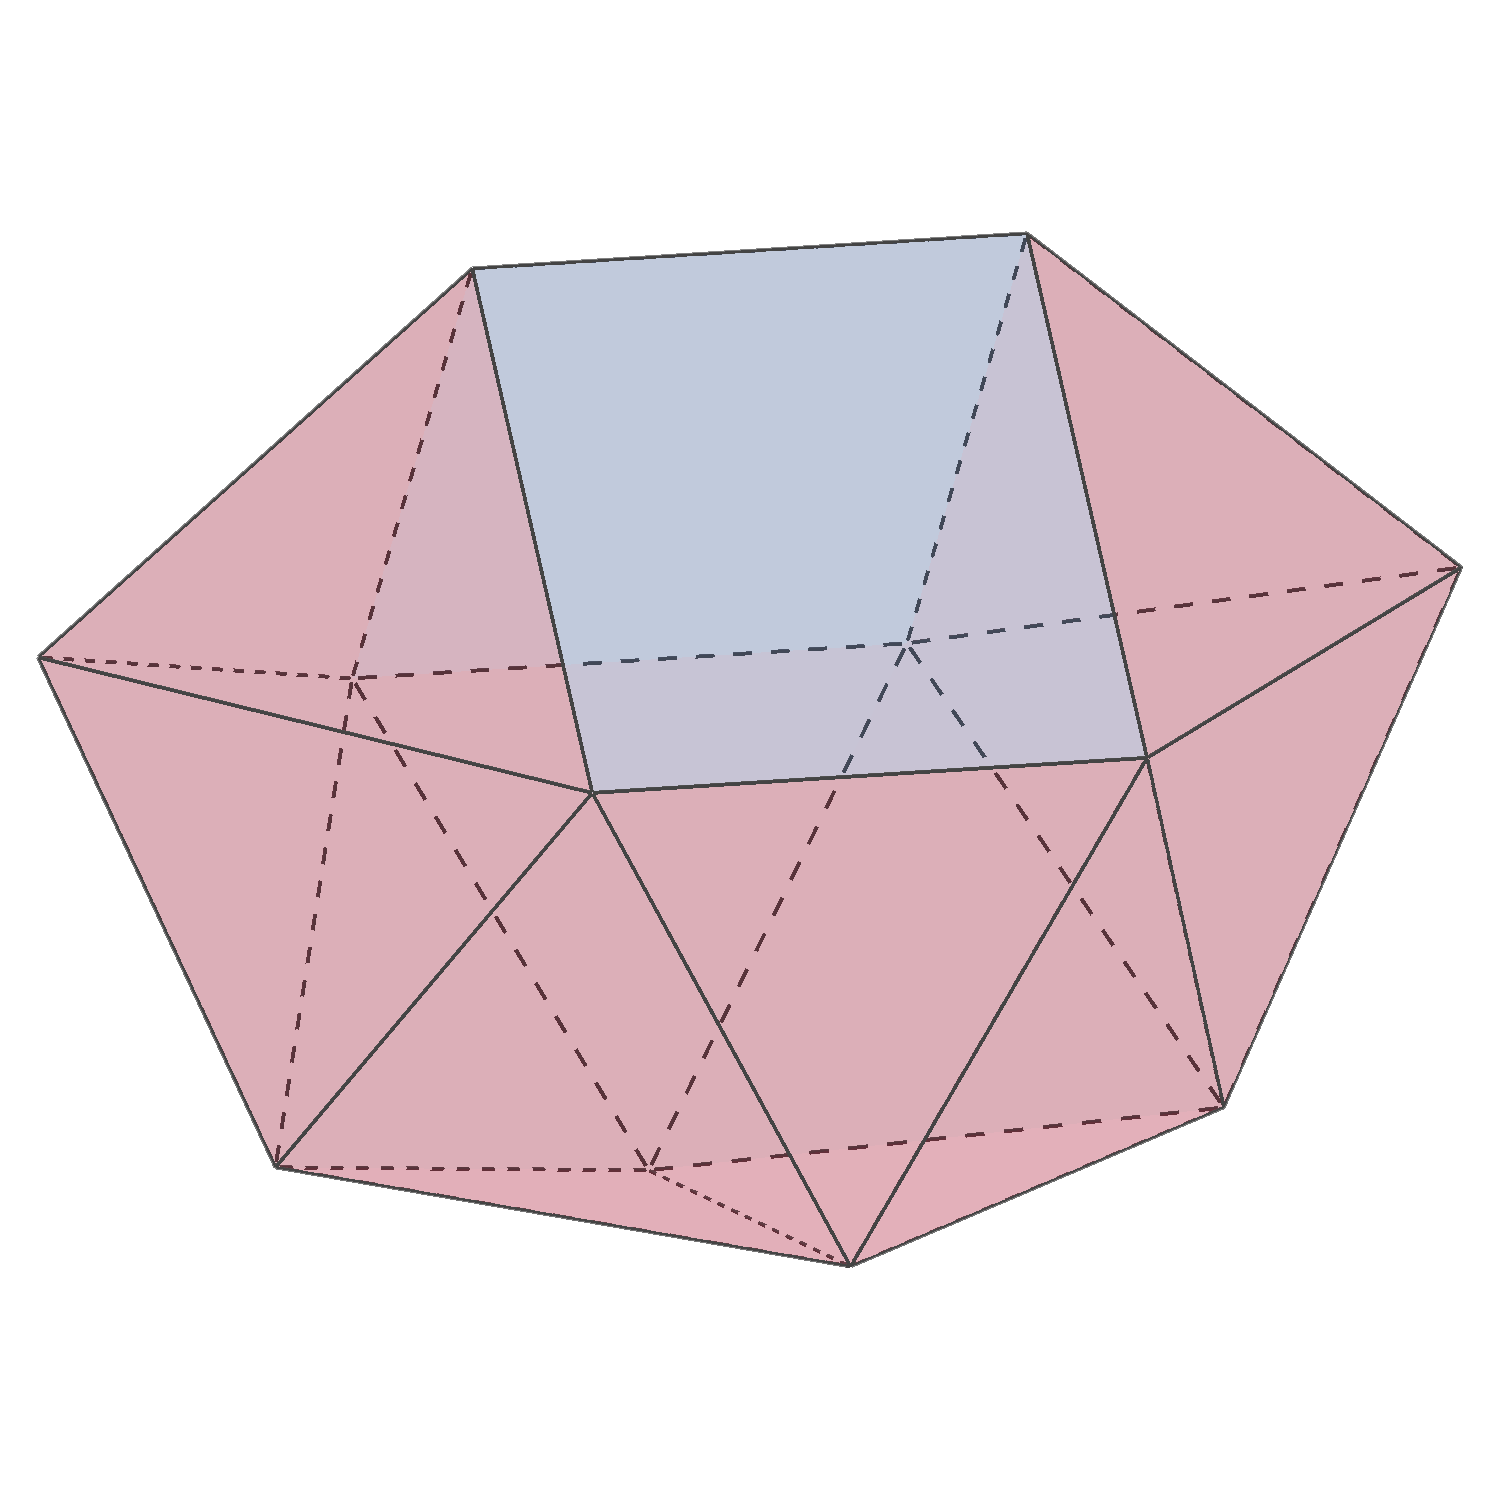
\includegraphics[width=.5\linewidth]{Sphenomegacorona}
    \caption{Sphenomegacorona}
    \label{fig:polyhedra_1}
  \end{subfigure}%
  \begin{subfigure}{.33333\textwidth}
    \centering
    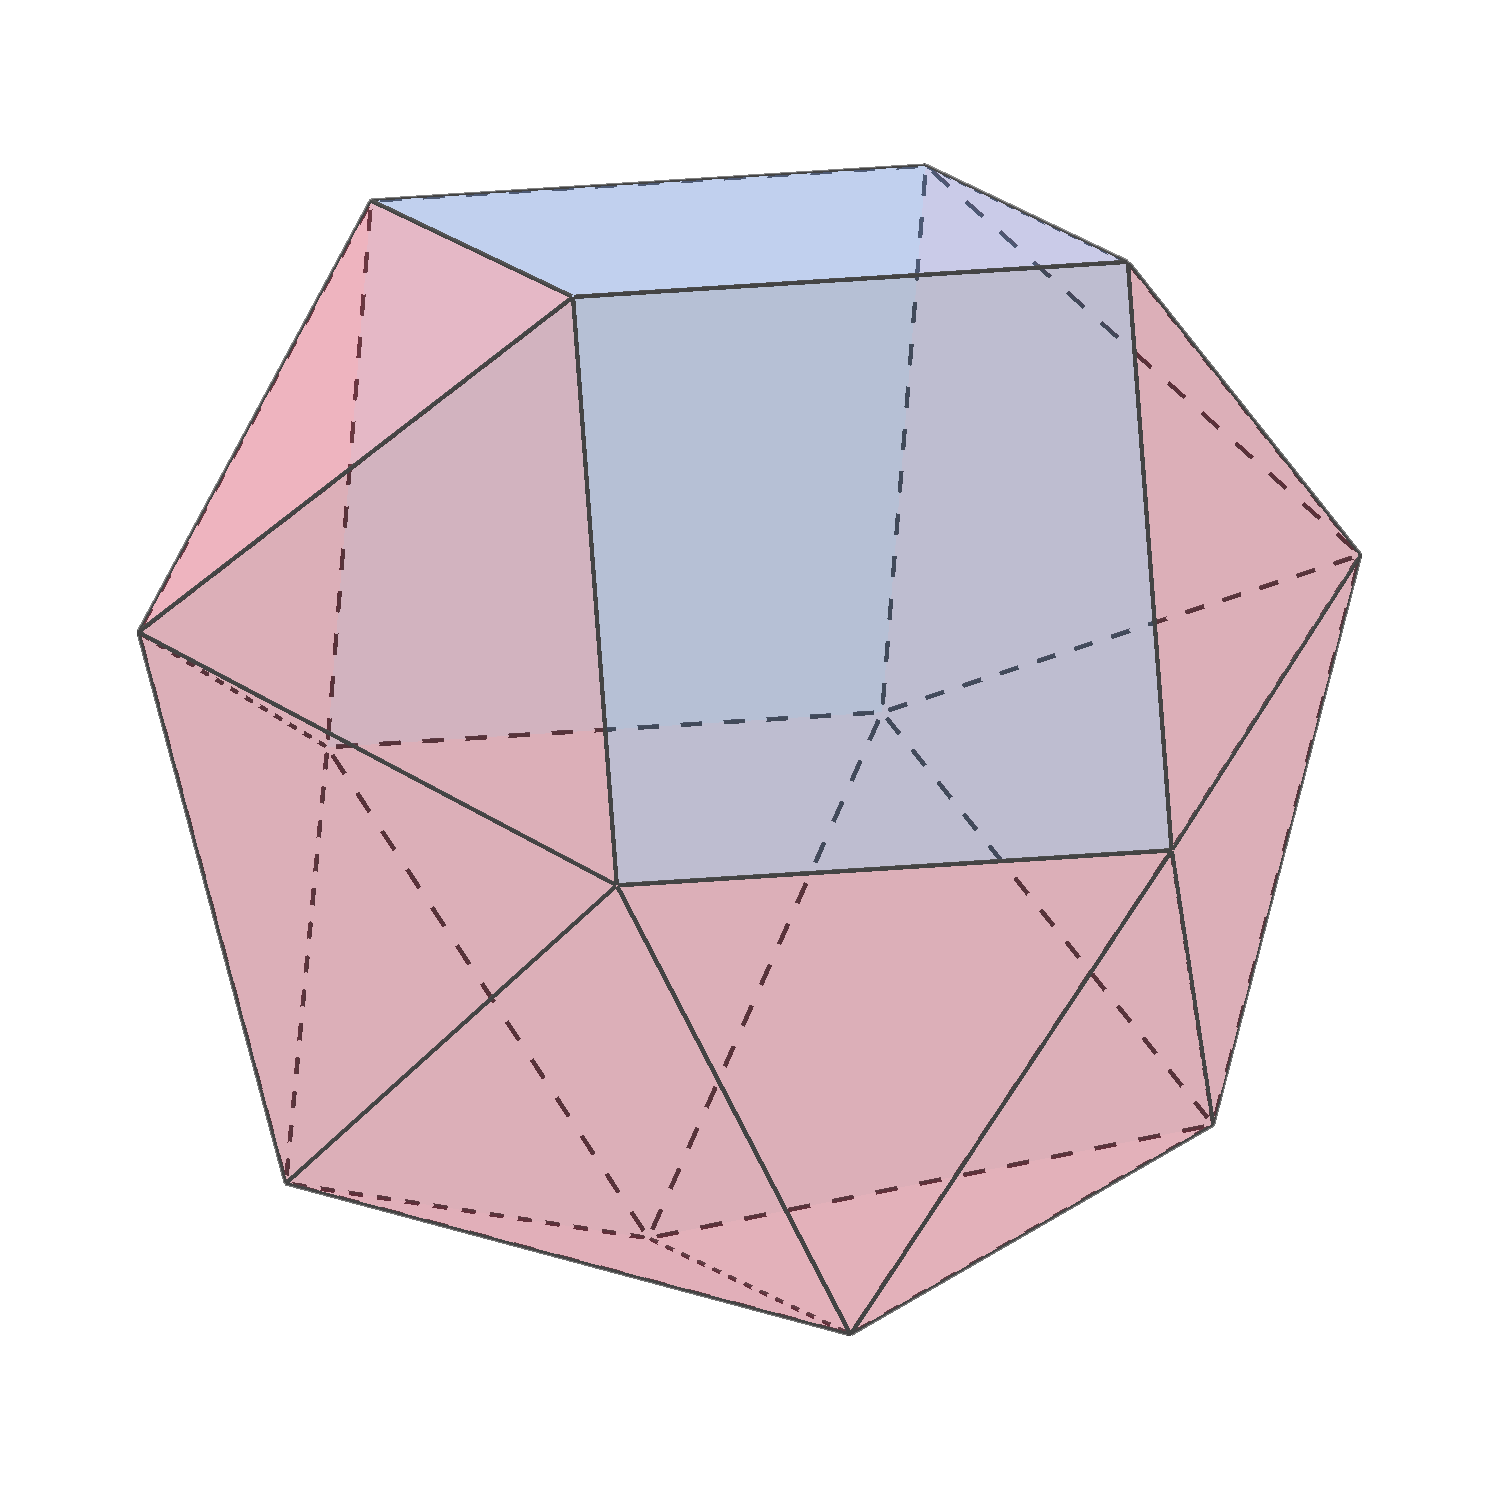
\includegraphics[width=.5\linewidth]{Hebesphenomegacorona}
    \caption{Hebesphenomegacorona}
    \label{fig:polyhedra_2}
  \end{subfigure}%
  \begin{subfigure}{.33333\textwidth}
    \centering
    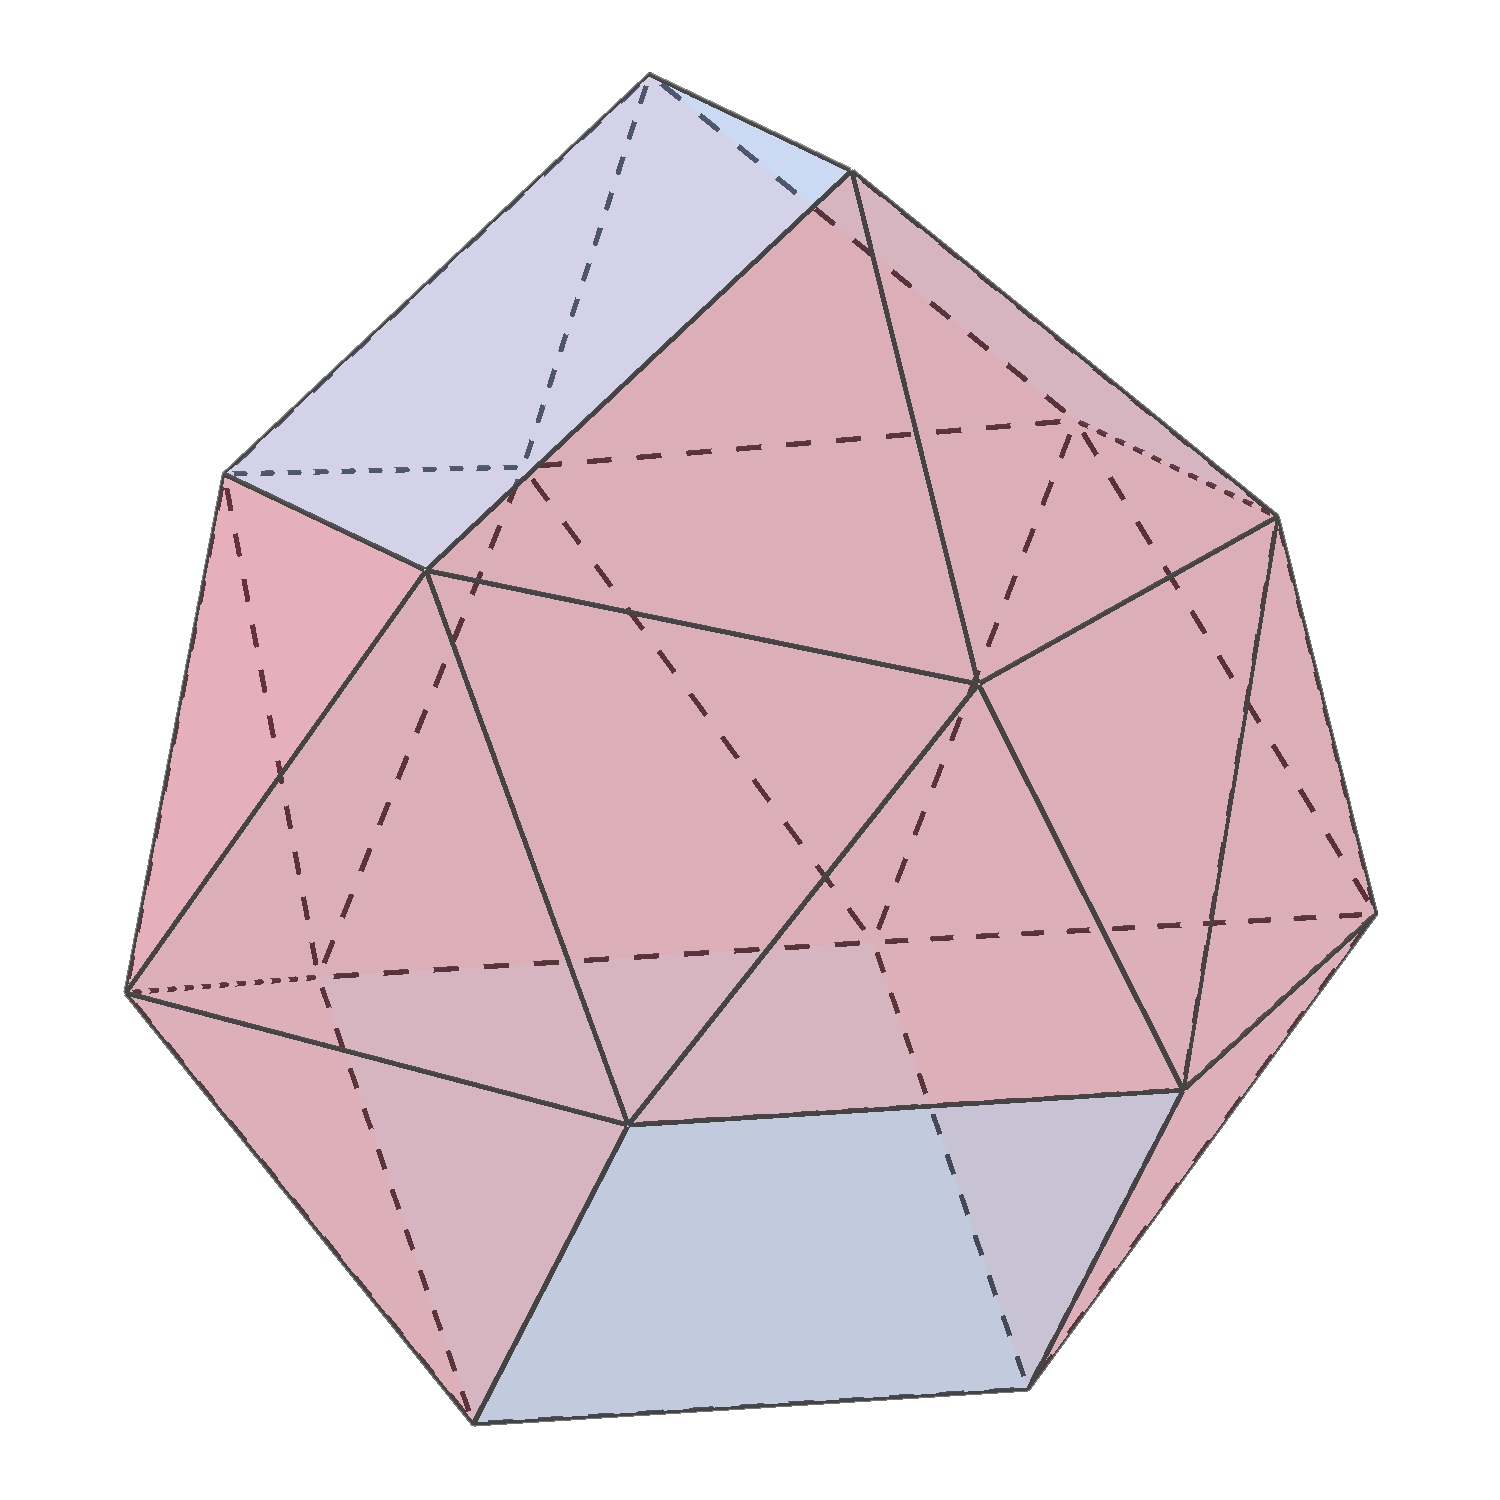
\includegraphics[width=.5\linewidth]{Disphenocingulum}
    \caption{Disphenocingulum}
    \label{fig:polyhedra_3}
  \end{subfigure}%
  \caption{Test images!}
  \label{fig:crf_polyhedra}
\end{figure}

The CRF polyhedra that are not also uniform are called the \textbf{Johnson solids}, named after
Norman Johnson who enumerated all 92 of them.

In 4D and up, the count of CRF polytopes explodes. There's thought to be at least about $10^{16}$
% Is this number accurate?
non-uniform CRF polychora. Because of this, people usually study subsets of CRFs.

\subsection{Scaliform polytopes}
\label{scaliform}

\textbf{Scaliformity} is a less strict version of uniformity. It does not require that
all facets are uniform, only that all edges are the same length.\footnote{
  It still requires isogonality of course.}

In 3D, the scaliform polytopes are the same as the uniform polytopes, because all the polygons
that can be faces of a scaliform polyhedron are regular and thus uniform.\footnote{
  For a detailed explanation, see Section \ref{circum}.} But there are
polyhedra, such as some of the Johnson solids\footnote{See Section \ref{crf}.}, that can be facets
of scaliform polychora. So scaliform polytopes are distinct from uniform polytopes in 4D and up.

\begin{figure}[H]
  \centering
  \includegraphics[width=.3\linewidth]{tut=invtut.png}
  \caption{One of the easiest to understand scaliform polytopes is the polychoron
    \textit{truncated tetrahedral alterprism}. It consists of two truncated tetrahedra
    in opposite orientations, their faces are connected by triangular cupolae, and
    their edges are connected by tetrahedra. It is not uniform because it has non-uniform
    facets (the triangular cupolae), but it is still isogonal and equilateral, thus it is
    scaliform.}
\end{figure}

\section{Useful terms}

\subsection{Vertex figure}
\label{verf}

A \textbf{vertex figure}, or \textbf{verf} for short, is a polytope that shows how
the facets of another polytope are arranged around a vertex. Intuitively, it can
be understood as the shape that gets exposed when you slice off a vertex of a polytope.

\begin{figure}[H]
  \centering
  \includegraphics[width=.3\linewidth]{cube_verf.png}
  \caption{The verf of a cube is a triangle. The edges of the triangle are
  themselves verfs of the faces of the cube.}
\end{figure}

A vertex figure has 1 less dimension than the original polytope. Verfs of polyhedra are
polygons, verfs of polychora are polyhedra, etc.

The facets of a vertex figure are the vertex figures of the facets of the original polytope,
and generally the elements of a vertex figure are the vertex figures of the elements of the
original polytope.

\section{In-depth definitions}
\label{indepth}

This section explains in detail some terms and definitions. If you're just starting out, you
don't need to care about this.

\subsection{Polytope}

As with many terms used on the Polytope Discord,
the word ``polytope'' can have a few definitions which are not completely equivalent.
This section will list four properties of a polytope from least to most controversial.
The most common definition is the strictest, requiring all four.
\begin{enumerate}
  \item
A polytope in $n$ dimensions (known hereafter as an $n$-polytope)
is made of \textbf{facets} which are $(n-1)$-polytopes.
\begin{itemize}
  \item \textbf{Points} ($0$-polytopes) are the facets of \textbf{line segments} ($1$-polytopes),
  \item which are the facets of \textbf{polygons} ($2$-polytopes),
  \item which are the facets of \textbf{polyhedra} ($3$-polytopes),
  \item which are the facets of \textbf{polychora} ($4$-polytopes), etc.
\end{itemize}

Note that an $n$-polytope must lie in $n$-dimensional space.
A square with a vertex jutting out of the plane is usually not a bona fide polygon
but is instead given the name ``\textbf{skew} polygon.''
If the skew square is a face of a larger 3D shape,
said 3D shape is not considered a polyhedron either,
since its faces are not all polygons.
Readers coming from jan Misali's video on regular polyhedra may find fault with this,
but the fact of the matter is that
skew polytopes are rarely mentioned or included in our lists.

For the next criterion, consider the following figures ABC and DEF.
\end{enumerate}

\begin{center}
  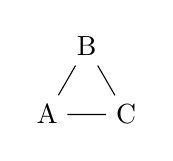
\begin{tikzpicture}
    \node (a) at (0,0) {A};
    \node (b) at (0.5,0.866) {B};
    \node (c) at (1,0) {C};
    \draw (a) -- (b) -- (c) -- (a);
  \end{tikzpicture}
  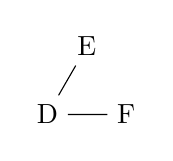
\begin{tikzpicture}
    \node (d) at (0,0) {D};
    \node (e) at (0.5,0.866) {E};
    \node (f) at (1,0) {F};
    \draw (e) -- (d) -- (f);
  \end{tikzpicture}
\end{center}

ABC is a triangle, a polygon with three line segments, or \textbf{edges},
as they are known when mentioned as part of a larger polytope.
It also contains three points, or \textbf{vertices}, or even \textbf{verts} for short.
(In the polytope world, abbreviations are everywhere!)
DEF, on the other hand, is not a triangle; it is missing an edge,
leaving ``open ends'' at E and F which are each connected to only one edge.
To exclude DEF and figures like it,
we require that within a polygon, every vertex be connected to exactly two edges.
This condition also excludes ``branches'' where more than two edges meet at a vertex.

Let's generalize this rule to $n$-polytopes.
Two 3D figures are shown below.

\begin{center}
  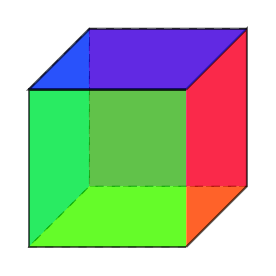
\begin{tikzpicture}
    \coordinate (A0) at (1,1,1);
    \coordinate (A1) at (1,1,-1);
    \coordinate (A2) at (1,-1,1);
    \coordinate (A3) at (1,-1,-1);
    \coordinate (A4) at (-1,1,1);
    \coordinate (A5) at (-1,1,-1);
    \coordinate (A6) at (-1,-1,1);
    \coordinate (A7) at (-1,-1,-1);
    \draw[dashed,fill=cyan,opacity=0.6] (A4) -- (A5) -- (A7) -- (A6);
    \draw[dashed,fill=magenta,opacity=0.6] (A1) -- (A5) -- (A7) -- (A3);
    \draw[dashed,fill=yellow,opacity=0.6] (A2) -- (A6) -- (A7) -- (A3);
    \draw[thick,fill=red,opacity=0.6] (A0) -- (A1) -- (A3) -- (A2);
    \draw[thick,fill=green,opacity=0.6] (A0) -- (A4) -- (A6) -- (A2);
    \draw[thick,fill=blue,opacity=0.6] (A0) -- (A4) -- (A5) -- (A1);
  \end{tikzpicture}
  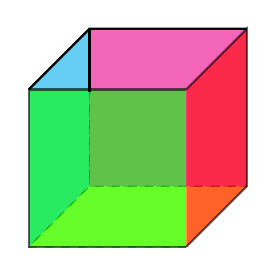
\begin{tikzpicture}
    \coordinate (A0) at (1,1,1);
    \coordinate (A1) at (1,1,-1);
    \coordinate (A2) at (1,-1,1);
    \coordinate (A3) at (1,-1,-1);
    \coordinate (A4) at (-1,1,1);
    \coordinate (A5) at (-1,1,-1);
    \coordinate (A6) at (-1,-1,1);
    \coordinate (A7) at (-1,-1,-1);
    \draw[dashed,fill=cyan,opacity=0.6] (A4) -- (A5) -- (A7) -- (A6);
    \draw[dashed,fill=magenta,opacity=0.6] (A1) -- (A5) -- (A7) -- (A3);
    \draw[dashed,fill=yellow,opacity=0.6] (A2) -- (A6) -- (A7) -- (A3);
    \draw[thick,fill=red,opacity=0.6] (A0) -- (A1) -- (A3) -- (A2);
    \draw[thick,fill=green,opacity=0.6] (A0) -- (A4) -- (A6) -- (A2);
    \draw[thick] (A4) -- (A5) -- (A1);
    \draw[thick] (A5) -- (-1,0.2,-1);
  \end{tikzpicture}
\end{center}

The left figure is a cube, a polyhedron with
six square \textbf{faces}, twelve edges, and eight vertices.
The right is the same, but with the top face removed.
The right figure is not a polyhedron because, like DEF, it leaves ``open ends.''
However, in this case, the open ends are not vertices but the top four edges,
which are each connected to only one face.
We require that within a polyhedron, every edge be connected to exactly two faces.\footnote{
  The previous rule for polygons does not apply to the cube nor to other polyhedra;
  every vertex of the cube is connected to three edges, not two.
  However, the rule does apply to each of the cube's square faces.
}

Are you beginning to see a pattern?
In an $n$-polytope, removing an $(n-1)$-dimensional facet
creates ``open ends'' in the $(n-2)$-dimensional ``facets of facets,'' or \textbf{ridges}.
Ridges are the vertices of polygons, the edges of polyhedra, the faces of polychora, and so on.
Thus the next trait of a polytope is:
\begin{enumerate}
  \setcounter{enumi}{1}
  \item Every ridge must be connected to exactly two facets.
\end{enumerate}
Collectively, a polytope's vertices, edges, faces,
and so on are known as its \textbf{elements}.
We may keep track of which elements have which others as facets using a \textbf{Hasse diagram},
shown below for the triangle ABC.

\begin{center}
  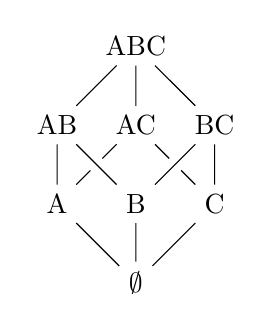
\begin{tikzpicture}
    \node (abc) at (0,3) {ABC};
    \node (ab) at (-1,2) {AB};
    \node (ac) at (0,2) {AC};
    \node (bc) at (1,2) {BC};
    \node (a) at (-1,1) {A};
    \node (b) at (0,1) {B};
    \node (c) at (1,1) {C};
    \node (o) at (0,0) {$\emptyset$};
    \draw (o) -- (a) -- (ab) -- (abc) -- (ac) -- (c)
    (b) -- (o) -- (c) -- (bc) -- (abc)
    (a) -- (ac);
    \draw[preaction={draw=white, -,line width=6pt}] (ab) -- (b) -- (bc);
  \end{tikzpicture}
\end{center}

Each node of the Hasse diagram represents an element of ABC,
including both the whole triangle at the top
and the \textbf{null element} $\emptyset$ at the bottom.\footnote{
  $\emptyset$, also known as the \textbf{nullitope}, is a convenient edge case.
  It has no vertices or other elements and is considered to be $-1$-dimensional.
}
Whenever two nodes of the diagram are connected,
the higher node's element contains the lower node's element as a facet.
For example, the edge AC contains the vertex C,
so their nodes are connected in the diagram with AC above C.
Notice that the structure of the diagram does not depend on
where the vertices of the original figure are;
a scalene triangle would have the same Hasse diagram as the equilateral ABC.

A diagram on its own, without the locations of the vertices,
is also known as an \textbf{abstract polytope}.
For example, consider the following diagram:

\begin{center}
  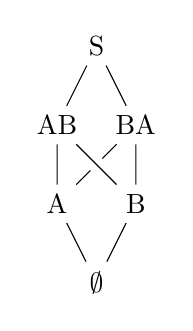
\begin{tikzpicture}
    \node (s) at (0,3) {S};
    \node (ab) at (-0.5,2) {AB};
    \node (ba) at (0.5,2) {BA};
    \node (a) at (-0.5,1) {A};
    \node (b) at (0.5,1) {B};
    \node (o) at (0,0) {$\emptyset$};
    \draw (o) -- (a) -- (ab) -- (s) -- (ba) -- (b) -- (o)
    (a) -- (ba);
    \draw[preaction={draw=white, -,line width=6pt}] (b) -- (ab);
  \end{tikzpicture}
\end{center}

It represents an abstract ``polytope'' with
one null element, two vertices, two edges, and one face (reading from the bottom up).
It satisfies the two conditions given thus far and is often called the digon (two-sided polygon).
However, its two edges AB and BA contain the same vertices
and will lie on top of each other when drawn on a sheet of paper.
For this reason, the digon is not considered a polytope.
Likewise, a quadrilateral with two vertices in the same spot,
which would look like a triangle when drawn, is also not a polytope.
This leads us to the third criterion:

\begin{enumerate}
  \setcounter{enumi}{2}
  \item No two elements of a polytope may coincide:
  \begin{enumerate}
    \item no two elements (other than vertices and $\emptyset$) may have the same facets and
    \item no two vertices may have the same location.
  \end{enumerate}
\end{enumerate}

Figures which pass the first and second tests but not this third,
such as the digon, are called \textbf{fissaries}.
Note than condition 3(b) is the first which cannot be tested just from the Hasse diagram.
Condition 1 is equivalent to requiring that the Hasse diagram be organized into ``layers,''
with one element on the top (the whole polytope) and another on the bottom ($\emptyset$).

Finally, perhaps the most contentious part of the definition: 

\begin{enumerate}
  \setcounter{enumi}{3}
\item
  A polytope is \textit{connected}, i.e.
  it is possible to reach any facet from any other facet
  by repeatedly jumping to adjacent facets.
  \footnote{
    Here, ``adjacent'' means ``sharing a ridge,''
    e.g. two edges of a polygon which share a point,
    or two faces of a polyhedron which share an edge.
  }
\end{enumerate}

Two triangles next to each other a polygon do not make!
Figures which fail to satisfy this criterion are known as \textbf{compounds}.
The question ``Are compounds polytopes?'' sparked lively discussusions
the first few times it was brought up on the server
and weary sighs thereafter.
With that, the definition of a polytope is complete!
\footnote{
  Perhaps the most common requirement for a polytope seen elsewhere but not here
  is convexity: not having dents, holes, or self-intersections.
  All of those are perfectly fine and, in fact, overwhelmingly common.
}

\subsection{Regular polytopes and flags}
\label{flag}

If you ask a server member what a regular polytope is,
they might reply ``a regular polytope is \textbf{flag-transitive}.''
This raises two questions: what is a flag, and what is ``-transitive?''
To answer the first question, reconsider the Hasse diagram of triangle ABC from earlier.
A flag of the triangle is a sequence of elements that starts with $\emptyset$ and ends with ABC,
where each entry in the sequence contains the previous one.
In other words, a flag is a path drawn through the diagram from bottom to top.
For example, $\emptyset$ $\rightarrow$ B $\rightarrow$ AB $\rightarrow$ ABC is a flag.
ABC happens to have six of them:
starting from $\emptyset$, there are three choices of vertex,
then two choices of which other vertex to include in the edge,
then only one choice of ABC as the final element.

Next, what is ``-transitive?''
Note that I keep the hyphen
because ``transitivity'' on its own is not a property;
something needs to come before the word.
A polytope is $x$-transitive if
every $x$ of the polytope can be moved to any other $x$
by some combination of rotation, reflection, and occasionally translation,
so that the polytope as a whole looks the same afterward.
For example, the following hexagon is vertex-transitive (or \textbf{isogonal}),
but not edge-transitive.

\begin{center}
\includegraphics[scale=0.1]{isogonal_hexagon.png}
\end{center}

Any of the six black vertices (intersection points don't count!)
can be moved to any other vertex with rotation or reflection.
However, an orange edge cannot be moved to a red one
without changing the shape, size, or orientation of the hexagon.

\subsection{Circumscribability and orbiformity}
\label{circum}

A $n$-polytope is \textbf{circumscribable} if its vertices lie on a $n-1$-sphere.
For a polygon, this means they lie on a circle, for a polyhedron, a sphere.

All elements of an isogonal spherical polytope are circumscribable. Take the example of
faces of a polyhedron: all the vertices of the polyhedron are equivalent and thus lie on a
sphere. A face of a polyhedron lies on a plane, and any intersection of a plane and a sphere
is a circle. So the vertices of the face lie on a circle. This works in any dimension.

A polytope is \textbf{orbiform} if it is circumscribable and all its edges are the same length.
Examples are all scaliform (including uniform) polytopes, some of the Johnson solids\footnote{
  See Section \ref{crf}.} and higher-dimensional CRF polytopes, and many nonconvex regular-faced
polytopes. All orbiform polygons are regular.

All elements of a scaliform polytope are orbiform.

\end{document}
